\section{Introduction}
L'objectif de ce TP	est de se familiariser avec les outils de simulation de distributions gaussiennes et leurs visualisation. Ceci sera fait à travers l'utilisation du package R \textbf{mvtnorm}. Il offre la possibilité de paramétrer la distribution, dans notre cas multivariée, selon un vecteur de moyennes $\mu$ et une matrice de variance/co-variance $\sigma$. Ce rapport se composera de deux parties, la première sera consacrée aux simulations de distributions et l'analyse de l'impacte de la variation des paramètres (distribution de moyennes, matrice de variance/co-variance, degré de mélange des distributions, proportions des classes, etc) sur chaque jeux de données. La deuxième partie sera quant à elle consacrée à l'étude d'un classifieur linéaire et d'un classifieur quadratique appliquées sur chacun des jeux de données généré au préalable. Une conclusion générale clôturera ce travail accompagné d'un résumé des points abordés.


\section{Simulation des jeux de données}
\paragraph{}
Nous nous intéresserons dans cette partie à l'étude de trois jeux de données générés suite à l'utilisation de la librairie \textbf{MixSim}. Ils sont caractérisés par :
\begin{itemize}
	\item \textbf{La forme des classes} : la forme de la distribution des individus, ou points, d'un point de vue géométrique. C'est à dire qu'elles soient sphériques ou allongés
	\begin{figure}[H]
		\centering
		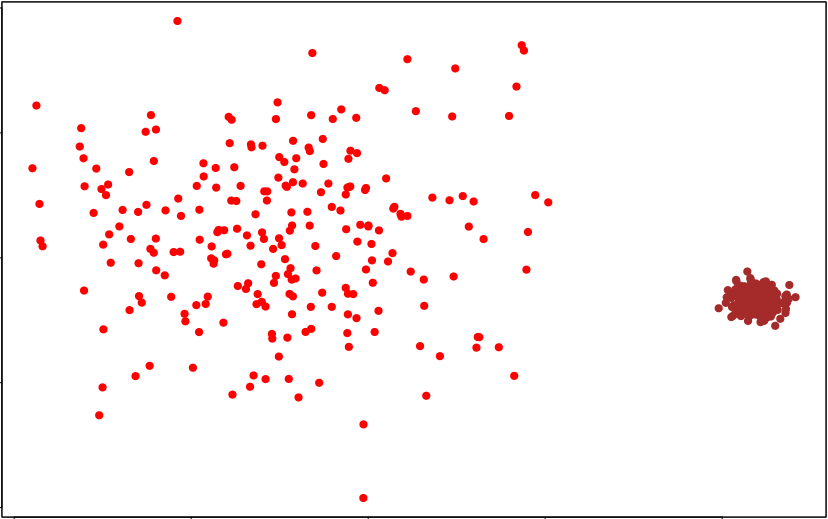
\includegraphics[width=0.5\linewidth]{images/spherical_classes.png}
		\caption{Deux classes sphériques bien séparées (Jeu de donnés I)}
		\label{fig:spherical}
	\end{figure}
	
	\item \textbf{Le degré de mélange des classes} : c'est à dire a quel point certains points d'une distribution appartiennent à plusieurs classes en même temps, les deux classes sont donc confondues dans une certaines régions de leur espace de représentation.
	
	\begin{figure}[H]
		\centering
		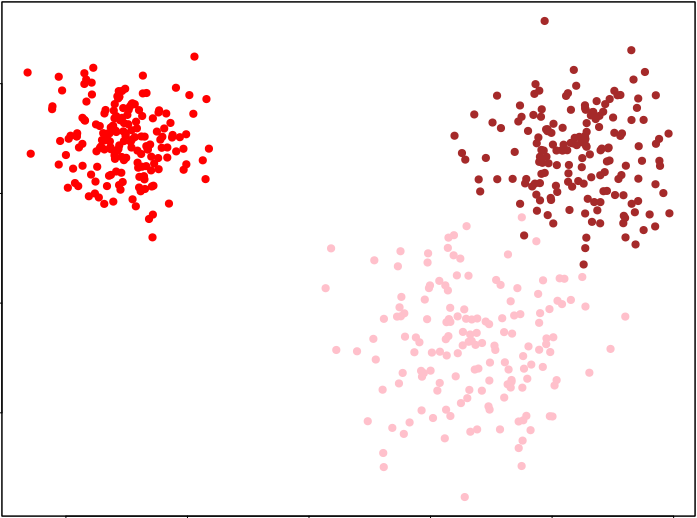
\includegraphics[width=0.5\linewidth]{images/spherical_classes_mixed.png}
		\caption{Trois classes sphériques mélangées à un degré $\bar{\omega} = 0.05$ (Jeu de donnés II)}
	\end{figure}

	\begin{figure}[H]
		\centering
		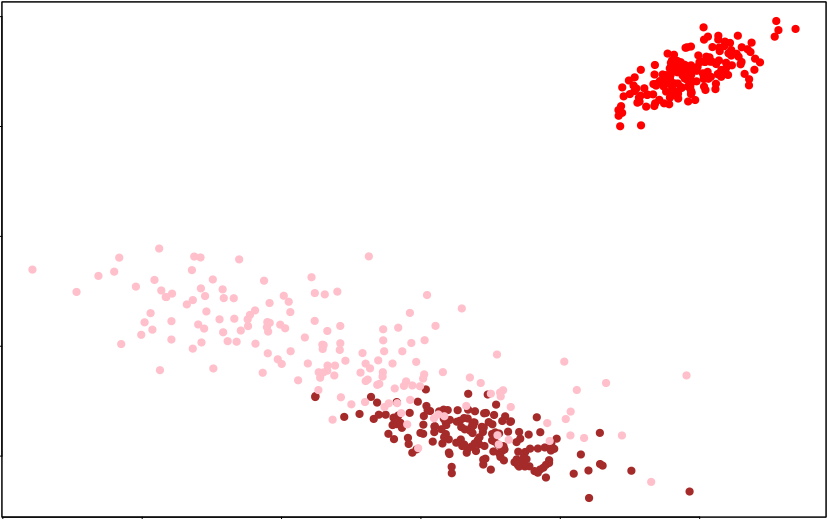
\includegraphics[width=0.5\linewidth]{images/non_spherical_classes_mixed.png}
		\caption{Trois classes non sphériques mélangées à un degré $\bar{\omega} = 0.05$ (Jeu de donnés III)}
	\end{figure}
\end{itemize}

\section{Fonction discriminante}
\paragraph{}
Avant d'entamer l'étude distributionnelle des différents jeux de données, nous allons introduire la fonction discriminante $G_i(x)$ avec $i\in{1,2,3}$ qui permettra, selon certaines hypothèses, de classifier un individu $x$. Pour rappel la fonction possède l'expression suivante : 
\begin{equation*}
	G_i(x) = -0.5*(x-\mu_i)^t \times \Sigma_i^{-1} \times (x-\mu_i) - 0.5 * \log{\Sigma_i} + \log{P(c_i)}
\end{equation*}
avec : 
\begin{itemize}
	\item $i$ : l'indice de la classe dont la fonction va tester la probabilité de contenance de l'individu $x$.
	\item $x$ : le vecteur à $p$ dimensions associé à l'individu à classer.
	\item $\mu_i$ : le vecteur à $p$ dimensions des moyennes de chaque variables sur l'ensemble de la classe $i$
	\item $\Sigma_i$ la matrice de variance/co-variance de taille $p \times p$ associée à la classe $i$
	\item $P(c_i)$ la probabilité a priori d'appartenance à la classe $i$
\end{itemize}
	\par
	La classification se fera donc en calculant la valeur de cette fonction pour un individu données pour chaque classe $i$, la valeur de $i$ correspondant à la valeur maximum de la fonction discriminante sera donc la classe que prédit le modèle. L'algorithme suivant résumé le procédé 
	\par 
	\begin{algorithm}[H]
		\KwIn{$x$ l'instance à classifier,
			 $mu_X$ : Matrice des moyennes,
			 $\Sigma_X$ : Tenseur des matrices de variance/co-variance,
		 	 $P_X^i$ : Vecteur des probabilités a priori}
		\KwOut{La classe de l'instance $x$}
		
		$max = g = G_i(x,\mu_X^i, \Sigma_X^i,P_X^i)$\;
		$max_i = 1$\;
		\For{$i \gets 2$ \textbf{to} $nb_classes$} {
			$g = G_i(x,\mu_X^i, \Sigma_X^i,P_X^i)$\;
			\If{$g > max$} {
				$max = g$\;
				$max_i =i$
			}
		}
		\Return{$max_i$}\;
		\caption{Classifier une instance $x$ selon la fonction discriminative $G$}
		\label{algo:predict}
	\end{algorithm}
	
\subsection{Jeu de données I}
\paragraph{}
Ce jeu de donnés assez basique est composé de $500$ individus caractérisés par deux variables $X_1$ et $X_2$ et divisés en deux classes bien distinctes de formes sphériques. l'une des classe est très condensée, ce qui peut se traduire par une faible variance de la distribution, voir la figure \ref{fig:spherical} et le tableau \ref{tab:var_c2}. Contrairement aux points de l'autre classe qui sont un peu plus éparpillés dans l'espace. La matrice de variance représentée par le tableau \ref{tab:var_c1} possède des éléments diagonaux dont les valeurs sont supérieures à ceux de la matrice associée à la classe $c_2$.
\begin{table}[ht]
	\begin{minipage}[b]{0.45\linewidth}\centering
		\begin{tabular}{|c|c|c|}
			\hline
			\textbf{}   & \textbf{X1}  & \textbf{X2}  \\ \hline
			\textbf{X1} & 0.01755423 & 0            \\ \hline
			\textbf{X2} & 0            & 0.01755423 \\ \hline
		\end{tabular}
		\caption{Matrice de variance/co-variance de la classe $c_1$ du jeu de données I}
		\label{tab:var_c1}
	\end{minipage}
	\hspace{0.5cm}
	\begin{minipage}[b]{0.45\linewidth}
		\centering
		\begin{tabular}{|c|c|c|}
			\hline
			\textbf{}   & \textbf{X1}  & \textbf{X2}  \\ \hline
			\textbf{X1} & 0
			
			.0002146625 & 0            \\ \hline
			\textbf{X2} & 0            & 0.0002146625 \\ \hline
		\end{tabular}
		\caption{Matrice de variance/co-variance de la classe $c_2$ du jeu de données I}
		\label{tab:var_c2}
	\end{minipage}
\end{table}
	\par
	Après avoir généré le jeu de données, nous avons entamé l'étude de la classification de l'échantillon généré. Pour cela il suffit de comparer la classe prédite en utilisant l'algorithme \ref{algo:predict}. Le résultat est résumé dans la matrice de confusion ci dessous.
	\begin{table}[H]
		\centering
		\begin{tabular}{|l|l|l|}
			\hline
			\textbf{}   & \textbf{$\hat{c_1}$} & \textbf{$\hat{c_2}$} \\ \hline
			\textbf{$c_1$} & 243         & 0           \\ \hline
			\textbf{$c_2$} & 0           & 257         \\ \hline
		\end{tabular}
		\caption{Matrice de confusion par rapport au jeu de données I}
	\end{table}
	\par
	Du fait que les classes soient assez bien séparées à la base, le classifieur n'aura pas de mal pour discriminer les deux classes. Ce qui explique le taux de classification parfait de $100\%$
	
\subsection{Jeu de données II}
	\paragraph{}
	Ce jeu de données se compose aussi de $500$ individus caractérisés par les mêmes deux variables $X_1$ et $X_2$ mais cette fois ci divisés en trois classes dont deux ont un certains degré d'ambiguïté. Elles sont donc mélangée à un certains degré $\bar{\omega}$. La forme sphérique des classes est aussi préservée. les trois classes sont moyennement dispersé comparé au jeu de données I. ce qui peut se traduire par une variance modérée des deux variables, voir la figure \ref{fig:spherical} et le tableau \ref{tab:var_c2}.
	
	
	
	\begin{table}[ht]
		\begin{minipage}[b]{0.45\linewidth}\centering
			\begin{tabular}{|c|c|c|}
				\hline
				\textbf{}   & \textbf{X1}  & \textbf{X2}  \\ \hline
				\textbf{X1} & 0.003131377 & 0            \\ \hline
				\textbf{X2} & 0            & 0.003131377 \\ \hline
			\end{tabular}
			\caption{Matrice de variance/co-variance de la classe $c_1$ du jeu de données II}
			\label{tab:var_c12}
		\end{minipage}
		\hspace{0.5cm}
		\begin{minipage}[b]{0.45\linewidth}
			\centering
			\begin{tabular}{|c|c|c|}
				\hline
				\textbf{}   & \textbf{X1}  & \textbf{X2}  \\ \hline
				\textbf{X1} & 0.006314948 & 0            \\ \hline
				\textbf{X2} & 0            & 0.006314948 \\ \hline
			\end{tabular}
			\caption{Matrice de variance/co-variance de la classe $c_2$ du jeu de données II}
			\label{tab:var_c22}
		\end{minipage}
	\end{table}
	\begin{table}[H]
		\centering
		\begin{tabular}{|l|l|l|}
			\hline
			\textbf{}   & \textbf{X1}  & \textbf{X2}  \\ \hline
			\textbf{X1} & 0.009892214 & 0            \\ \hline
			\textbf{X2} & 0            & 0.009892214 \\ \hline
		\end{tabular}
		\caption{Matrice de variance/co-variance de la classe $c_3$ du jeu de données II}
		\label{tab:var_c32}
	\end{table}
	\par
	De manière analogue au jeu de données I, le classifieur donne d'assez bons résultats, un taux de classification de $98.6\%$. Toutefois, le degré de mélange affecte négativement le taux de classification. En particulier, en examinant la matrice de confusion ci dessous, le classifieur confond souvent les classes mélangées.
	
		\begin{table}[H]
		\centering
		\begin{tabular}{|l|l|l|l|}
			\hline
			\textbf{}   & \textbf{$\hat{c_1}$} & \textbf{$\hat{c_2}$}  & \textbf{$\hat{c_3}$} \\ \hline
			\textbf{$c_1$} & 174         & 0           & 0           \\ \hline
			\textbf{$c_2$} & 0           & 163         & 6           \\ \hline
			\textbf{$c_3$} & 0         & 1           & 156           \\ \hline
			
		\end{tabular}
		\caption{Matrice de confusion par rapport au jeu de données II}
	\end{table}

	\subsection{Jeu de données III}
	\paragraph{}
	Ce jeu de données se compose lui aussi de $500$ individus caractérisés par les mêmes deux variables $X_1$ et $X_2$ cette fois ci aussi divisés en trois classes dont deux ont un différent degré d'ambiguïté quantifié par $\bar{\omega}$. Cependant, la forme sphérique des classes est délaissé au profit d'une forme plus allongé et elliptique. La variance varie d'une classe à une autre, ainsi on retrouve une densité dans les individus de la classe 2 qu'on ne retrouve pas forcement dans les deux classes restantes. Nous notons aussi l'apparition d'une covariance entre certaines variables des classes, principalement dû au fait que les classes ne soient pas totalement sphériques.
	
	
	
	\begin{table}[ht]
		\begin{minipage}[b]{0.45\linewidth}\centering
			\begin{tabular}{|c|c|c|}
				\hline
				\textbf{}   & \textbf{X1}  & \textbf{X2}  \\ \hline
				\textbf{X1} & 0.02478492 & -0.007431410            \\ \hline
				\textbf{X2} & -0.00743141            & 0.008072644 \\ \hline
			\end{tabular}
			\caption{Matrice de variance/co-variance de la classe $c_1$ du jeu de données III}
			\label{tab:var_c13}
		\end{minipage}
		\hspace{0.5cm}
		\begin{minipage}[b]{0.45\linewidth}
			\centering
			\begin{tabular}{|c|c|c|}
				\hline
				\textbf{}   & \textbf{X1}  & \textbf{X2}  \\ \hline
					\textbf{X1} & 0.005868395 & 0.005103484            \\ \hline
				\textbf{X2} & 0.005103484            & 0.010760323 \\ \hline
				
			\end{tabular}
			\caption{Matrice de variance/co-variance de la classe $c_2$ du jeu de données II}
			\label{tab:var_c23}
		\end{minipage}
	\end{table}
	\begin{table}[H]
		\centering
		\begin{tabular}{|l|l|l|}
			\hline
			\textbf{}   & \textbf{X1}  & \textbf{X2}  \\ \hline
		\textbf{X1} & 0.03558796 & 0.008045200            \\ \hline
		\textbf{X2} & 0.00804520            & 0.009474448 \\ \hline
		\end{tabular}
		\caption{Matrice de variance/coparticulier, en examinant la matrice de confusion ci dessous, le classifieur confond souvent les classes mélangées.-variance de la classe $c_3$ du jeu de données II}
		\label{tab:var_c33}
	\end{table}
	\par
	Le classifieur donne dans ce cas aussi d'assez bons résultats, un taux de classification de $91\%$. Mais le degré de mélange affecte de façon encore plus négative le taux de classification, l'ambiguïté se trouvant être plus accentué entre les classes mélangées comme le montre la matrice de confusion suivante.
	
	\begin{table}[H]
		\centering
		\begin{tabular}{|l|l|l|l|}
			\hline
			\textbf{}   & \textbf{$\hat{c_1}$} & \textbf{$\hat{c_2}$}  & \textbf{$\hat{c_3}$} \\ \hline
			\textbf{$c_1$} & 163         & 2           & 0           \\ \hline
			\textbf{$c_2$} & 0           & 160         & 6           \\ \hline
			\textbf{$c_3$} & 3         & 31           & 132           \\ \hline
			
		\end{tabular}
		\caption{Matrice de confusion par rapport au jeu de données III}
	\end{table}
	
	
\section{Conclusion}
\paragraph{}
Au terme de ce court TP, nous avons pu nous familiariser avec l'utilisation des outils de simulations présent dans R. L'étude réalisée sur ces simulations ont étés conformes a notre intuition scientifique. Nous avons pu observer, de manière assez simplifiée, la limite que doit faire face un modèle de discrimination linéaire. L'ambiguïté entre deux classes ainsi que la forme de ces dernières sont donc des points à ne surtout pas négliger pour le choix de cette méthode. 